%\usepackage[top=0.5cm,bottom=0.5cm,left=0.5cm,right=0.5cm]{geometry}
%\usepackage[a5paper,top=0cm,bottom=0cm,left=0cm,right=0cm]{geometry}
\documentclass{article}
\usepackage{listings}
\usepackage{color} %red, green, blue, yellow, cyan, magenta, black, white
\definecolor{mygreen}{RGB}{28,172,0} % color values Red, Green, Blue
\definecolor{mylilas}{RGB}{170,55,241}
\usepackage[swedish]{babel}
\usepackage[utf8]{inputenc}
\usepackage{amsmath}
\usepackage{graphicx}
\usepackage{float}
\usepackage{hyperref}
\usepackage{caption}
\usepackage{lipsum}
\usepackage{listings}
\usepackage{listingsutf8}
\usepackage{xcolor}
\usepackage{textcomp}
\usepackage{units}
\usepackage{bbm}
\usepackage{url}
\usepackage[swedish]{isodate}
\usepackage{gensymb}
\usepackage{amssymb}
\usepackage{amsthm}
\usepackage{fullpage}
\usepackage{tikz}
\usepackage{pgfplots} 
\usepackage{pgfgantt}
\usepackage{pdflscape}
\pgfplotsset{compat=newest} 
\pgfplotsset{plot coordinates/math parser=false}
\usepackage{todonotes}
\usepackage{siunitx}
\usepackage{geometry}
\usepackage[utf8]{inputenc}
\usepackage[T1]{fontenc}
\usepackage[swedish]{babel}
\usepackage{csquotes}
\usepackage{amsmath}
\usepackage{ae} 
\usepackage{units}
\usepackage[version=4]{mhchem}
\usepackage{icomma}
\usepackage{color}
\usepackage{graphicx}
\usepackage{bbm}
\usepackage{textcomp}
\usepackage{hyperref}
\usepackage{verbatim}
\usepackage{wrapfig}
%\usepackage{natbib}
\usepackage{multirow}
\usepackage{subfig}
\usepackage[titletoc]{appendix}
\usepackage{float}
\usepackage{parskip}
\usepackage{subfiles}
\newcommand{\HRule}{\rule{\linewidth}{0.5mm}}
\usepackage{chemfig} %https://en.wikibooks.org/wiki/LaTeX/Chemical_Graphics
\usepackage[
backend=biber,
style=ieee,
citestyle=numeric 
]{biblatex}
%https://www.tablesgenerator.com/
%https://www.codecogs.com/latex/eqneditor.php
\hbadness=10000
\addbibresource{references.bib}
%\addbibresource{timmie.bib}
 % här ligger även bra hemsidor som man kan använda
\begin{document}

\begin{titlepage}
\begin{centering}

{\huge\bfseries Vanadinutvinning från LD slagg som använts som syrebärare i förbränningsprocesser \par}
\vspace{1cm}
{\scshape\Large Projektsplanering \\ \textbf{KBTX-10-19-06}\par}
{\scshape\Large \par}
{\Large\itshape Timmie Dzafo Paulsson, Stefan Ewaldsson, \\ Victor Hernvall, Marcus Mellqvist \\ , Marcus Thim, Frida Tropp, .\par}
{\large \today\par}
%Ordna i ordning
{   \par}
{   \par}
{    \par}


%\begin{figure}[!ht]
%\centering
%
\includegraphics[scale=0.3]{chalmers.png}
%\label{fig:chalmers}

%\end{figure}
%\centering{\textbf{CHALMERS TEKNISKA HÖGSKOLA} \par}


\end{centering}
\end{titlepage}


\begin{centering}
\topskip15pt
\end{centering}
\newpage
\thispagestyle{empty}
\thispagestyle{empty}
\tableofcontents
\thispagestyle{empty}
\newpage
\pagenumbering{arabic}


%bakgrund 
% Börja med stålindustrin, masugn etc
% Teori LD-slagg
% Vanadin

% Förbränning
% Fluideserad bädd
% Syrebärare  
% Biomassa

% Hur de två länkar samman. 



\section{Bakgrund}
Vanadin, grundämne nummer 23, är en övergångsmetall i det periodiska systemets femte grupp. Vanadin hittas i en handfull olika tillämpningsområden som exempelvis katalysator i en rad olika tillverkningsprocesser\cite{Pecoraro2014}.
Metallen har oxidationstillstånd, +2,+3,+4 och +5,  \cite{Baroch2013} vilket har gjort att metallen varit av särskilt intresse i flödesbatterier och därför föremål för studier ända sedan förra århundradet\cite{Skyllas-Kazacos1987}.
Fördelen med de många oxidationstillstånden är att elektrolyterna i batteriets halvceller kan bestå av samma metall vilket är fördelaktigt med avseende på kontaminering av membran, elektrod och elektrolyter\cite{Lopez-Vizcaino2017}. Vanadin nyttjas dock i dagsläget mest som ett additiv i ståltillverkning vars syfte är att stärka stålet\cite{Baroch2013}.

I dagens samhälle ökar behovet av förnybar energi i form av exempelvis solkraft för att ersätta fossila alternativ. Detta yttrade sig tydligt i Sverige 2018 då intresset för solkraft ökade som ett svar på regeringens beslut om utökat investeringkostnadsstöd från 20 till 30 procent i solcellsinstallationer från och med den första januari 2018\cite{SverigesEnergimybn2009}.

Problemet som kvarstår är dock att förnyelsebara energikällor i allmänhet och solceller i synnerhet inte producerar elektricitet i paritet med efterfrågan; förnyelsebara elnät är överlag känsliga mot de fluktuationer som uppstår i elnätet. Lösningen på ett av dagens energiproblem skulle alltså kunna lösas genom att lagra energin med flödesbatterier av vanadintyp\cite{Lopez-Vizcaino2017}.


Vanadin lades i januari 2018 i EU:s lista över kritiska material under direktivet om en cirkulär ekonomi\cite{Navigation2018}. 
Som en följd av detta har företag som exempelvis Scandivanadium och EU Energy Corporation via Bergsstaten ansökt om undersökningstillstånd att utvinna just vanadin ur svenska mineralfyndigheter på Österlen i Skåne respektive utkanten av Östersund i Jämtland. Dessa beslut möts ej sällan av kontrovers där missnöje yttras genom protester från bofasta individer i områdena. \cite{NohrstedtLinda2018}. 
För att tackla problemet med att försöka uppnå en cirkulär ekonomi kan det därför finnas ett intresse i att utvinna vanadin på annan väg, nämligen deponerat LD-slagg istället för att bryta helt ny mineral.

\subsection{Stålslagg}
Vid framställning av stål bildas diverse restprodukter som exempelvis gasreningsstoft, gasreningsslam och just slagg. Gasreningsstoft är de små partiklar som följer med de gaser som bildas i ståltillverkningens varma processer. Dessa avskiljs i hög utsträckning tillsammans med rökgaser i diverse filtreringsanordningar. Stoften kategoriseras som torra eller våta och efter rening  bildar de gasreningsstoft respektive gasreningsslam. [Jernkontoret - Gasreningsstoft och -slam blir nya råvaror][Jernkontoret handbok] 

Stålslagg förekommer i en rad olika typer som t.ex. ljusbågsugnsslagg och LD-slagg\cite{Pehlke2014a}. %Nämn vad LD står för och varför! 
Slaggen kategoriseras utifrån vilken typ av ugn som använts vid framställning av råjärnet. Ljusbågsugnsslagg är restprodukt av skrotbaserad ståltillverkning medan LD-slagg är restprodukt i malmbaserad ståltillverkning\cite{Pehlke2014a}. Slagg kan brukas i diverse tillämpningar som exempelvis konstruktionsmaterial eller asfalt; detta för att minska uttaget av jungfruliga resurser. Dessutom använder Stålverken begagnat material som skrot för tillverkning av nya produkter; detta för att nyttja resurserna till sitt yttersta. [https://www.jernkontoret.se/sv/stalindustrin/tillverkning-anvandning-atervinning/restprodukter/slagg/][https://www.jernkontoret.se/sv/stalindustrin/tillverkning-anvandning-atervinning/atervinning-av-jarn-och-stal/] 

Svenskt ståls branschorganisation Jernkontoret hävdar trots detta att 20\% av avfallet, där spår av vanadin kan hittas, hamnar på deponi hos antingen kommunal deponeringsplats eller en extern aktör\cite{PontusWestrin}. Det tål också att nämnas att det finns tillgängligt flera ton av gammalt deponerat slagg till förfogande som syrebärare följt av lakmaterial. %Notera att man här inte vet vad varken en syrebärare eller ett lakmaterial är. Kanske ta bort meningen alternativt flytta ner den?

%[https://www.jernkontoret.se/sv/stalindustrin/tillverkning-anvandning-atervinning/restprodukter/]
%Båda dessa citerade 04-02-2019 

\subsection{Som syrebärare i förbränningsprocesser}
Det har visat sig att LD-slagg har potential som en billig syrebärare i kemcyklisk förbränning (CLC), där två stycken fluidiserande bäddreaktorer nyttjas för att separera CO$_2$ vid förbränning \cite{Xu2017}. Detta illustreras enligt Figur 1 %INFOGA! 
nedan. Syrebäraren, som i detta fallet är LD-slagg, oxideras i ena reaktorn genom tillförsel av syre. Denna förflyttas sedan till den andra reaktorn där bränslet reducerar LD-slagget, för tillbakaförsel till första reaktorn.  %Har freestylat detta. Glöm inte att jämföra med källa för att se så det stämmer!
 
Syrebärare kan även nyttjas i Oxygen Carrier Aided Combustion (OCAC), d.v.s. förbränning i en fluidiserad bädd där bäddmaterialet består av just en syrebärande metall.
Syftet är att transportera syre till bränslet i understökiometriska områden för att på så vis öka pannans effektivitet\cite{Zevenhoven2018}.
 
 Förbränning av biomassa är något som förknippas med CO$_2$ neutrala utsläpp och även i vissa fall negativa CO$_2$ utsläpp i de fall koldioxidlagring nyttjas som exempelvis en kemcyklisk förbränning\cite{Zevenhoven2018}.

Vid analys av LD-slagg som nyttjats som bäddmaterial i Chalmers 12 MW cirkulerad fluidiserad bädd-förbrännare hittades ett skal av vanadin och fosfor kring partiklarnas yttre hölje med SEM-EDX-teknik. Det finns skäl att testa om detta skulle kunna underlätta lakning av båda dessa komponenter.

\section{Syfte}
Syftet med arbetet är således att testa om lakning av LD-slagg som befunnit sig i en fluidiserad bädd är en tillfredsställande metod för utvinning. Detta skulle kunna stänga materialkretslopp med avseende på inte bara vanadin utan eventuellt också fosfor och LD-slaggets livstid skulle kunna förlängas gentemot dagens spann. När lakning har utförts kommer det också analyseras i vilka typer av lakningsbara faser vanadinet finns i och hur dessa skulle kunna tänkas efterbehandlas. 

\section{Problem}
Den huvudsakliga uppgiften består i att jämföra möjligheterna att utvinna vanadin ur LD-slag som har genomgått olika behandlingar innan lakning.

Deluppgift ett kommer bestå i att utföra en rad experiment som undersöker under vilka förhållanden och i vilket medium, d.v.s syra eller bas, som lakningen är mest gynnsam.

%ändra detta då vi bara kommer titta på syra i nuläget

Deluppgift 2 kommer vara att jämföra resultaten av utvinning av vanadin från LD-slag som är obearbetat och de som använts som syrebärare. Dessutom kommer det vara intressant att identifiera i vilka komplex vanadin förekommer. Detta kommer undersökas med hjälp av röntgendiffraktion.

Utöver de test som kommer göras för att analysera mängden utvunnen vanadin kommer det även testas vilken halt fosfor som erhålls i samma prov.
I mån av tid kan det även testas specifikt för fosfor och även ändra lakningsparametrar för att underlätta utvinningen av fosfor.
\newpage
\section{Metod}

Laborationerna kommer i största utsträckningen ske i grupper om tre och tre, utan att ha någon särskild indelning av personer. Utan det kommer snarare bero på vilka gruppmedlemmar som är tillgängliga. I början av varje vecka kommer ett möte att hållas för att planera den kommande veckan och se vad som gjordes föregående vecka. 

Valet av metod grundar sig i tidigare uppställningar för liknande laborationer, samt en laborations uppställning som visas av handledaren Duygu Yilmaz\cite{Aarabi-Karasgani2010}. Experimentuppställningen består av en 3-halsad kolv som befinner sig i ett vattenbad på en värmeplatta med magnetomrörning. Till de tre halsarna så är en av halsarna försedd med en kork, en med en termometer, och slutligen en med kondensor se Figur \ref{fig:lab}. Temperaturen, ration mellan vätska och fast ämne, samt koncentration på syran väljs beroende på vilken kedja av experiment som utförs, se tabell \ref{tab:metodtab}. Lakningen sker genom att 1 gram av LD-slagget tillsätts till H$_{2}$SO$_{4}$, som är förvärmt till rätt temperatur för det experimentet. Omrörningen har bestämts till 360 rpm. Provet lakas i 2 timmar och provtagningen sker i intervallerna 30 minuter, 60 minuter, 120 minuter. Vid provtagning plockas 5 ml upp av provet. Efter att lakningen är gjord så filteras provet med en Büchner tratt med ett glasfilter och ett pappersfilter. Provet är nu efter detta redo för att analyseras med en AAS. 

\begin{table}[H]
\caption{Premilinär test uppställning.}
\begin{tabular}{|l|c|c|c|}
\hline
\textbf{\begin{tabular}[c]{@{}l@{}}Parametrar\end{tabular}}              & \multicolumn{1}{l|}{\textbf{\begin{tabular}[c]{@{}l@{}}H$_{2}$SO$_{4}$ \\ koncentration [M]\end{tabular}}} & \multicolumn{1}{l|}{\textbf{\begin{tabular}[c]{@{}l@{}}Ratio mellan flytande \\ fast och  [ml/g]\end{tabular}}} & \multicolumn{1}{l|}{\textbf{\begin{tabular}[c]{@{}l@{}}Laknings\\ Temperatur  [$\degree$C]\end{tabular}}} \\ \hline
\textbf{\begin{tabular}[c]{@{}l@{}}H$_{2}$SO$_{4}$ \\ koncentration [M]\end{tabular}}    & 3,4,5                                                                                                    & 25:1                                                                                                           & 70                                                                                                        \\ \hline
\textbf{\begin{tabular}[c]{@{}l@{}}Ratio mellan flytande\\ och fast [ml/g]\end{tabular}} & 3                                                                                                          & 25:1, 30:1, 40:1                                                                                            & 70                                                                                                        \\ \hline
\textbf{\begin{tabular}[c]{@{}l@{}}Laknings \\ Temperatur  [$\degree$C]\end{tabular}}    & 3                                                                                                          & 25:1                                                                                                           & 50, 60, 70, 80                                                                                               \\ \hline
\end{tabular}
\label{tab:metodtab}
\end{table}

 Ett flertal metoder kommer att användas för att analysera proverna. Atomabsorptionsspektroskopi, AAS, och röntgenkristallografi, XRD från engelska X-ray diffraction, och svepelektronmikroskop, SEM. De olika metoderna används för olika delar av arbetet. AAS används för att undersöka om vanadin har lakats ur LD slagget. XRD kommer att användas för att analysera kristallstrukturen av LD slagget före och efter att det har rostats och vid olika intervaller under rostningen för att se sammansättningen av de olika ämnena i kristallen. Slutligen så kommer SEM användas för att se var i LD slagget som de olika ämnena befinner sig i slaggpartiklarna. 

Planeringen är att en litteraturstudie ska ske parallellt med laborationerna för att kunna ge möjlighet till djupare inlärning och förklaring av ämnet. Detta innebär användningsområden av vanadin, användadet av LD slagg och dess deponering i nuläget. Även vilka fördelar och nackdelar processen har och vad det kan göra för samhällsnytta inför i framtiden. 

\section{Avgränsningar}

%Även om det är ett ämnes område som det i nuläget redan görs forskning på, inom olika applikationer och djupare förståelse, så finns det mycket potential i det här projektet. Men det med begränsade resurser, främst tid, så kommer vi behöva göra en mängd avgränsningar på vad som kommer att kollas på. 

Liknande projekt som detta arbetas på i nuläget. Men de projekten rostar LD-slagget snarare än att använda det som en syrebärare i den fludiserade bädden av ett värmekraftverk. Då detta är en unik möjlighet så krävs det att avgränsningar sker tidigt för att kunna fokusera på ett spetsområde.  

Arbetet ha därför begränsats till att bara undersöka lakning med svavelsyra. Dessutom kommer endast tre olika parametrar undersökas, trots att det finns många fler som påverkar. Försöken kommer dessutom att vara en faktor i taget försök vilket medför en något bristfällig optimering. Tanken är att försöken ska ge en fingervisning om hurvida denna typ av lakning kan tänkas vara värd att fortsätta forska på.

%Det här arbetet kommer inte heller ta hänsyn till ekonomiska och kemitekiska optimeringar. Det innebär optimering av storskaliga system eller hur det ska tillämpas på en uppskallad process. Detta görs i avseende av att det är inte projektet syfte, samt att det kommer att innebära en ännu större litteraturstuide än vad som är planerat.


\section{Samhälleliga och etiska aspekter}
Det finns en  väldigt stor industri som tillämpar LD-processen för att tillverkar stål. Till följd av detta finns även en väldigt stor sidoström innehållande stålslagg, kallat LD-slagg. Detta slagg läggs i nuläget på deponi, vilket skulle kunna vara en negativ samhällelig aspekt om det hanteras illa. Det vill säga att deponin läggs på ett ställe där den blir skrymmande eller stör utsikten. 

En mer etisk aspekt av deponin vore i fallet att exempelvis tungmetaller och fosfor läcker ut i närliggande vattendrag eller jordmån.

Genom att använda LD-slagg som syrebärare i förbränningsprocesser och vidare laka den brända slaggen för utvinning av vanadin ger en hållbar och cyklisk process som utnyttjar restprodukter från en annan process som är lättillgänglig och finns i stora kvantiteter.

\section{Tidsplan}
Tidsplanen som skall följas finns lättöverskådligt i Appendix \ref{appendix}, där Figur \ref{fig:Ganttliten} är ett Gantt-schema som veckovis ger en överblick över projektet och Figur \ref{fig:Ganttroterad} är ett mer utförligt Gantt-schema på dagbasis för projektet. Schemat är preliminärt och viss ändring kan ske, exempelvis kan laborationsarbetet pågå längre än planerat eller avslutas tidigare beroende på hur labbarbetet kommer gå.

\newpage
\printbibliography
\thispagestyle{empty}
\newpage
\appendix
\section{Appendix} \label{appendix}
\pagenumbering{roman}
\begin{figure}[H]
    \centering
    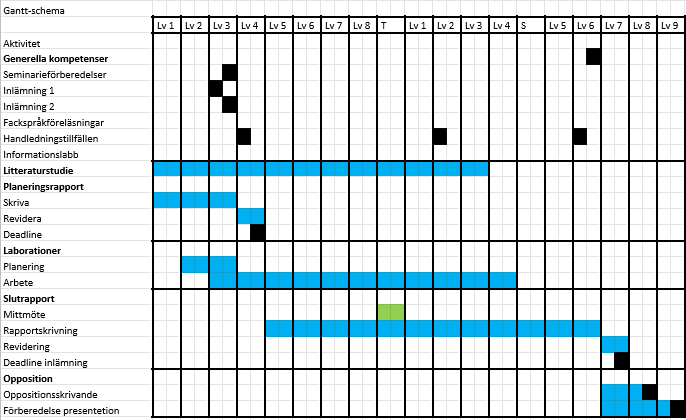
\includegraphics[scale=0.8]{Ganttliten.PNG}
    \caption{Gantt-schema över veckorna relaterat till projektbeskrivningen}
    \label{fig:Ganttliten}
\end{figure}

\newpage
\thispagestyle{empty}
\begin{figure}[H]
    \centering
    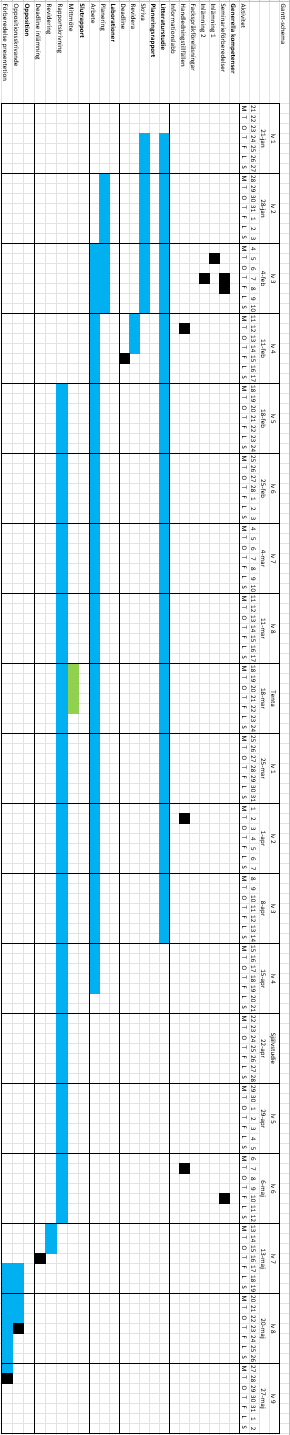
\includegraphics[scale=0.6]{Ganttroterad.PNG}
    \caption{Gantt-schema över hela projektet, dag för dag}
    \label{fig:Ganttroterad}
\end{figure}

\newpage
\thispagestyle{empty}
\begin{figure}[H]
    \centering
    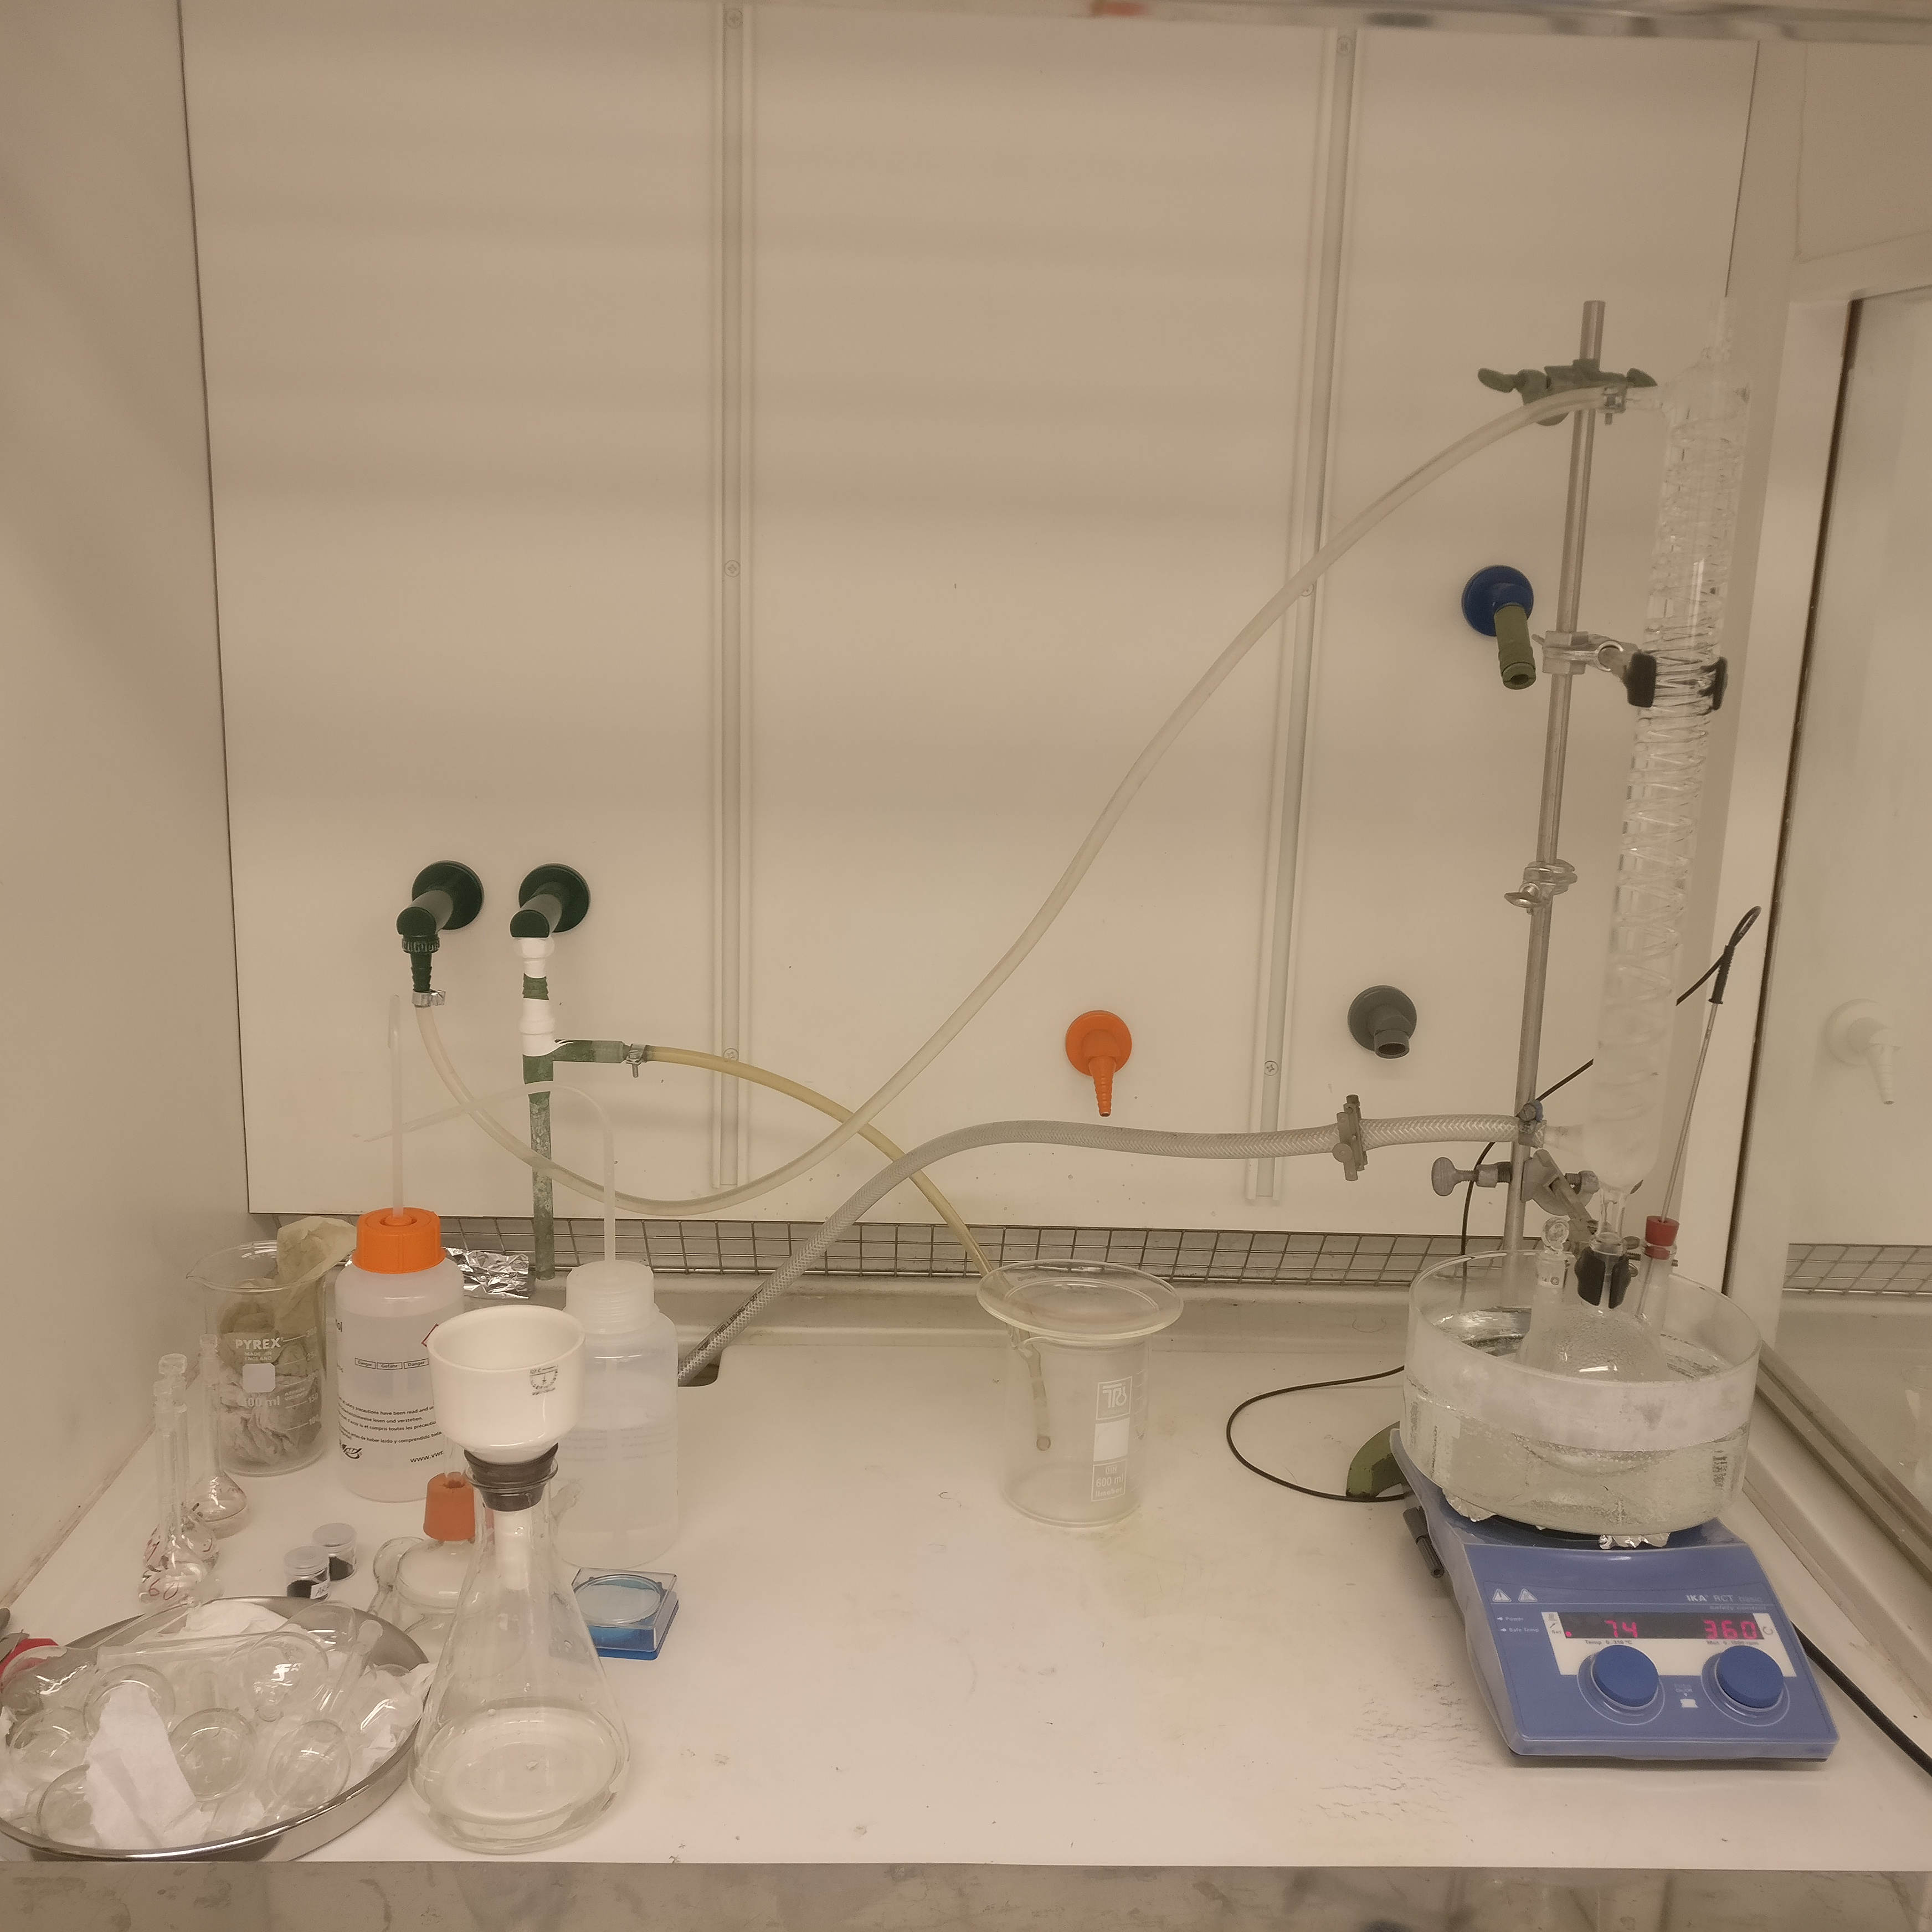
\includegraphics[scale=0.1]{labsetup.jpg}
    \caption{Laborations uppställningen i nuläget.}
    \label{fig:lab}
\end{figure}

\end{document}

